\chapter{HASIL DAN PEMBAHASAN}
\label{hasil-dan-pembahasan}
Bangunan yang dijadikan objek penelitian adalah \textit{climate chamber} DTNTF FT UGM. Dalam bab ini, akan dibahas mengenai hasil perancangan sistem kontrol sesuai dengan langkah-langkah yang dijelaskan pada Bab IV dengan memvariasikan berbagai macam masukan, kemudian mengetahui keluarannya. Variasi masukan dan keluaran akan dimodelkan dengan model jaringan saraf tiruan untuk mendapatkan parameter-parameter model yang dapat mengendalikan sistem bangunan.

\section{Hasil Pengembangan Model Plant JST}

Penulis menggunakan model JST yang telah dibangun oleh Tri Hartanto\cite{skripsiTanto} sebagai model acuan dalam penelitian ini. Model tersebut kemudian penulis kembangan kembali untuk mengingkatkan kinerjanya sebagai model \textit{plant}. \textit{Hyperparameter} yang digunakan Tri Hartanto pada pembangunan model plant JST ini dijelaskan pada Tabel \ref{tbl:5:NNPlantTanto}.\\

\begin{table}[!h]
	\caption{Tabel Rancangan Model Plant JST Tri Hartanto}
	\label{tbl:5:NNPlantTanto}
	\centering
	% use packages: array
	\begin{tabular}{|p{5.7cm}|p{5cm}|}
		\hline
		\textbf{Nama Hyperparameter} & \textbf{Nilai Hyperparameter} \\ \hline
		Arsitektur & Feedforward Neural Network \\ \hline
		Pembagian Data & 50\% 25\% 25\% \\ \hline 
		Jumlah Layar Tersembunyi & 1 \\ \hline
		Jumlah Neuron pada Layar & [55] \\ \hline
		Fungsi Aktivasi Layar & Hyperbolic Tangent \\ \hline
		Algoritma Pembelajaran & Levenberg-Marquardt \\ \hline
		Mean Absolute Error (MAE) & Td: 0,59$^\circ$C ; RH: 5,44\% \\ \hline
		Mean Squared Error (MSE) & Td: 0,75$^\circ$C ; RH: 52,33\% \\ \hline
		Koefisien Korelasi (R) & Td: 96,23\% ; RH: 68,90\% \\ \hline
	\end{tabular}
\end{table}
\vspace{2em}

%Tri Hartanto membangun model \textit{plant} dengan menggunakan data menyeluruh selama 24 jam. Pada penelitian ini penulis membangun model dengan menggunakan data selama jam operasional, yaitu pukul 07:00 s.d. 17:00. Hal ini dilakukan karena pada praktiknya \textit{climate chamber} digunakan untuk pengujian pada jam operasional tersebut. Hasil model \textit{plant} dengan penyesuaian data ini dapat dilihat pada Tabel \ref{tbl:5:NNPlantTanto2}.

Berdasarkan Tabel \ref{tbl:5:NNPlantTanto}, penulis melihat kinerja model yang lebih baik yang digambarkan dengan nilai MAE dari model tersebut. MAE untuk model yang telah disesuaikan bernilai lebih kecil dari model yang dikembangkan Tri Hartanto. Bahkan kinerja model cukup signifikan terhadap variabel kelembapan relatif.\\

\noindent \textbf{Hasil Variasi Pembagian Data} 

Dalam menentukan variasi pembagiaan data, penulis melakukan perbandingan dengan beberapa variasi pembagiaan data ke dalam 5 variasi. Kemudian, penulis membandingkan kinerja dari setiap pembagian data dengan menggunakan model JST dengan konfigurasi \textit{hyperparameter} sesuai rancangan penelitian sebelumnya\cite{skripsiTanto}.

\begin{table}[h!]
	\caption{Daftar variasi pembagian data}
	\label{tbl:5:DataSplitting}
	\centering
	% use packages: array
	\begin{tabular}{|p{3cm}|p{3cm}|p{1.5cm}|p{1cm}|p{1.5cm}|p{1cm}|}
		\hline
		Pembagian Data   & Persentase Data \\ \hline
		Data Splitting 0 & (50\% 25\% 25\%)\\ \hline
		Data Splitting 1 & (60\% 20\% 20\%)\\ \hline
		Data Splitting 2 & (70\% 15\% 15\%)\\ \hline
		Data Splitting 3 & (80\% 10\% 10\%)\\ \hline
		Data Splitting 4 & (80\% 15\% 05\%)\\ \hline
		Data Splitting 5 & (85\% 10\% 05\%)\\ \hline
	\end{tabular}
\end{table}

\begin{figure}[!h]
	\centering
	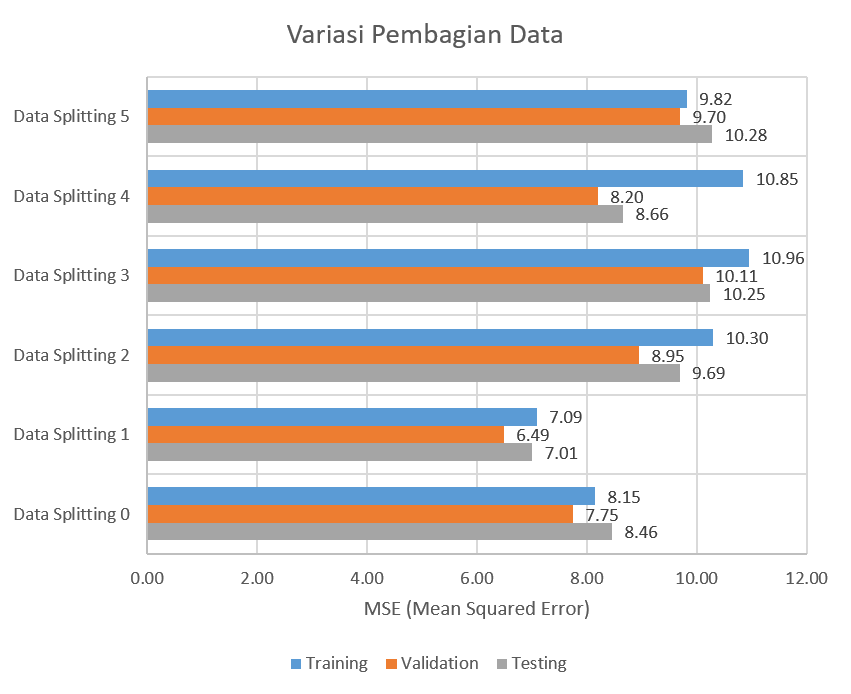
\includegraphics[width=0.9\textwidth]{figures/DataSplittingResult}
	\caption{Hasil Variasi Pembagian Data}
	\label{fig:5:DataSplittingResult}
\end{figure}

Pada Tabel \ref{tbl:5:DataSplitting}, "Data Splitting 0" merupakan konfigurasi pembagian data yang digunakan oleh Tri Hartanto pada penelitian sebelumnya dalam membangun model plant JST. Pada tabel yang penulis sajikan, penulis menulis pembagian data dengan format 'Data Splitting n' dan '(x\% y\% z\%)' dimana n = nomor variasi, x = pembagian data pelatihan, y = pembagian data validasi, dan z = pembagian data pengujian. Pembagian data terbaik yang penulis gunakan yaitu pembagian data bernama "Data Splitting 4". Data dibagi menjadi 3 bagian, yakni 80\% data pelatihan, 15\% data validasi, dan 5\% data pengujian. Sehingga didapatkan rancangan terbaik penulis yang dirangkum pada Tabel \ref{tbl:5:NNPlantRidhan}.\\

\begin{figure}[!h]
	\centering
	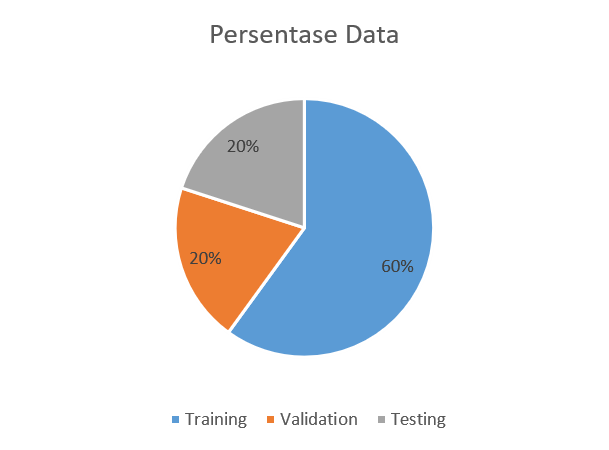
\includegraphics[width=0.75\textwidth]{figures/DataSplittingFinal}
	\caption{Pembagian Data yang digunakan}
	\label{fig:5:DataSplittingFinal}
\end{figure}
\vspace{1em}

\begin{table}[!h]
	\caption{Tabel Rancangan Model Plant JST Penulis}
	\label{tbl:5:NNPlantRidhan}
	\centering
	% use packages: array
	\begin{tabular}{|p{5.7cm}|p{5cm}|}
		\hline
		\textbf{Nama Hyperparameter} & \textbf{Nilai Hyperparameter} \\ \hline
		Arsitektur & Feedforward Neural Network \\ \hline
		Pembagian Data & 85\% 15\% 5\% \\ \hline 
		Jumlah Layar Tersembunyi & 1 \\ \hline
		Jumlah Neuron pada Layar & [55] \\ \hline
		Fungsi Aktivasi Layar & Hyperbolic Tangent \\ \hline
		Algoritma Pembelajaran & Levenberg-Marquardt \\ \hline
		Mean Absolute Error (MAE) & Td: 0,62$^\circ$C ; RH: 5,45\% \\ \hline
		Mean Squared Error (MSE) & Td: 0,82$^\circ$C ; RH: 54,45\% \\ \hline
		Koefisien Korelasi (R) & Td: 93,09\% ; RH: 71,44\% \\ \hline
	\end{tabular}
\end{table}

Dari pengembangan model plant JST ini, penulis mendapatkan rancangan yang lebih baik lagi dari hasil kinerja rancangan sebelumnya. Dengan mengubah pembagiaan data dari 50\% 25\% 25\% ke 85\% 15\% 5\%, nilai MAE model untuk kelembapan raltif pun berubah menjadi sebesar 0,62$^\circ$C untuk suhu ruang dan 5,45\% untuk kelembapan relatif.

\section{Hasil Perancangan Sistem Kontrol JST}

Berdasarkan diagram blok sistem kontrol pada Gambar \ref{fig:4:ConstrolSystemBlockDiagram}, penulis menggunakan Internal Model Control sebagai Sistem Kontrol JST dengan komponen emulator JST (\textit{NN Forward Model}) dan kontroler JST (\textit{NN Inverse Model}) di dalamnya. Pada sub-bab ini penulis juga akan menjabarkan hasil kinerja dari sistem kontrol pada simulasi simulink.

\subsection{Kinerja Emulator JST}

Penulis menggunakan \textit{NN Forward Model} sebagai emulator pada sistem kontrol. Model ini mirip seperti rancangan model plant JST yang dijelaskan pada sub-bab sebelumnya. Perbedaannya berada pada masukan dan keluaran dari arsitektur JST yang digambarkan pada Gambar \ref{fig:4:NNForwardModelDesign}. Hasil kinerja emulator JST ini dijabarkan pada Tabel \ref{tbl:5:NNEmulator}

\begin{table}[!hbt]
	\caption{Tabel Rancangan Emulator JST (\textit{NN Forward Model})}
	\label{tbl:5:NNEmulator}
	\centering
	% use packages: array
	\begin{tabular}{|p{5.7cm}|p{5cm}|}
		\hline
		\textbf{Nama Hyperparameter} & \textbf{Nilai Hyperparameter} \\ \hline
		Arsitektur & Feedforward Neural Network \\ \hline
		Pembagian Data & 80\% 15\% 5\% \\ \hline 
		Jumlah Layar Tersembunyi & 1 \\ \hline
		Jumlah Neuron pada Layar & [55] \\ \hline
		Fungsi Aktivasi Layar & Hyperbolic Tangent \\ \hline
		Algoritma Pembelajaran & Levenberg-Marquardt \\ \hline
		Mean Absolute Error (MAE) & Td: 0,51$^\circ$C ; RH: 1,43\% \\ \hline
		Mean Squared Error (MSE) & Td: 0,49$^\circ$C ; RH: 5,91\% \\ \hline
		Koefisien Korelasi (R) & Td: 96,38\% ; RH: 97,79\% \\ \hline
	\end{tabular}
\end{table}

\subsection{Kinerja Kontroler JST}

Penulis menggunakan \textit{NN Inverse Model} sebagai kontroler pada sistem kontrol. Pada proses pelatihan JST, penulis melakukan pengskalaan terhadap semua input JST menggunakan metode \textit{Min Max Scaling} kecuali variabel delay umpan masuk SET AC dan SET Heater. Pengskalaan bertujuan untuk meningkatkan kinerja JST menjadi optimal dengan menyamakan rentang dan besar satuan dari setiap variabel. Masing-masing variabel diubah menjadi skala satuan dengan melakukan transformasi data secara statistik. Data dari setiap variabel akan dikurangi dengan nilai minimum variabel tersebut yang dikemudian dibagi oleh selisih dari nilai maksimum dan nilai minimum variabel tersebut. Secara lengkap dapat dirumuskan pada persamaan berikut:
\begin{equation} \label{eq:5:MinMaxScaler}
z = \frac{x_i - min(x)}{max(x) - min(x)}
\end{equation}

Rancangan kontroler JST mirip dengan rancangan model plant JST. Perbedaannya hanyalah pada jumlah neuron pada \textit{hidden layer} yang berjumlah 52 neuron. Hasil kinerja dari kontroler JST ini dapat dilihat pada Tabel \ref{tbl:5:NNControler}.

\begin{table}[!h]
	\caption{Tabel Rancangan Kontroler JST (\textit{NN Inverse Model})}
	\label{tbl:5:NNControler}
	\centering
	% use packages: array
	\begin{tabular}{|p{5.7cm}|p{5cm}|}
		\hline
		\textbf{Nama Hyperparameter} & \textbf{Nilai Hyperparameter} \\ \hline
		Arsitektur & Feedforward Neural Network \\ \hline
		Pembagian Data & 85\% 15\% 5\% \\ \hline 
		Jumlah Layar Tersembunyi & 1 \\ \hline
		Jumlah Neuron pada Layar & [52] \\ \hline
		Fungsi Aktivasi Layar & Hyperbolic Tangent \\ \hline
		Algoritma Pembelajaran & Levenberg-Marquardt \\ \hline
		Mean Absolute Error (MAE) & AC: 0,23$^\circ$C ; HT: 0,00 \\ \hline
		Mean Squared Error (MSE) & AC: 4,85$^\circ$C ; HT: 0,00 \\ \hline
		Koefisien Korelasi (R) & AC: 98,41\% ; HT: 99,64\% \\ \hline
	\end{tabular}
\end{table}

\hfill\break
\hfill\break

\subsection{Kinerja Sistem Kontrol JST}

Sistem kontrol yang dijalankan penulis menghasilkan kinerja yang cukup baik untuk mengendalikan suhu ruang dan kelembapan relatif.

\begin{figure}[!h]
	\centering
	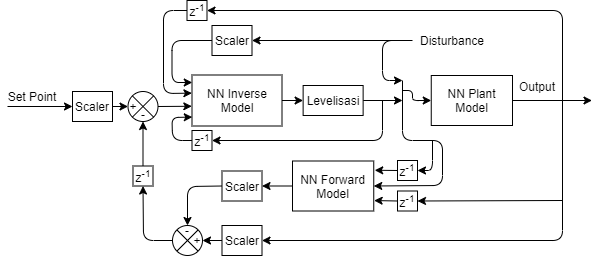
\includegraphics[width=0.9\textwidth]{figures/ControlDesignDiagram}
	\caption{Blok Diagram Sistem Kendali JST}
	\label{fig:5:ConstrolSystemBlockDiagram}
\end{figure}

\subsubsection{SET POINT Konstan SP1}

Kombinasi SET Point dapat dilihat pada Tabel \ref{tbl:5:SP1Combination}. Hasil dari simulasi simulink dapat dilihat pada Gambar \ref{fig:5:SimulinkSP1Td} dan Gambar \ref{fig:5:SimulinkSP1RH}. Pada Gambar \ref{fig:5:SimulinkSP1Td} dan Gambar \ref{fig:5:SimulinkSP1RH} dapat dilihat bahwa nilai \textit{error steady-state} sistem kontrol cukup kecil. Nilai \textit{Error Steady-State} dari simulasi ini dapat dilihat pada Tabel \ref{tbl:5:SP1Ess}. Grafik dari hasil simulasi dapat dilihat pada Gambar \ref{fig:5:SimulinkSP1Td} untuk Suhu Ruang dan Gambar \ref{fig:5:SimulinkSP1RH} untuk Kelembapan Relatif. Kontroler mengeluarkan nilai \textit{Manipulated Variable} yang ditunjukkan oleh Gambar \ref{fig:5:SimulinkSP1AC} dan Gambar \ref{fig:5:SimulinkSP1HT}.\\

\vspace{0.5em}
\begin{table}[!h]
	\caption{Nilai Kombinasi SET POINT SP1}
	\label{tbl:5:SP1Combination}
	\centering
	% use packages: array
	\begin{tabular}{|l|c|}
		\hline
		\textbf{Variabel} & \textbf{SET Point} \\ \hline
		Suhu Ruang (Td) & 26$^\circ$C          \\ \hline
		Kelembapan Relatif (RH) & 90\%         \\ \hline
		Suhu Luar (To) & 27$^\circ$C           \\ \hline
		Radiasi Matahari (RD) & 400 W/m$^2$    \\ \hline
	\end{tabular}
\end{table}

\vspace{0.5em}
\begin{table}[!h]
	\caption{Hasil Simulasi Sistem Kontrol SP1}
	\label{tbl:5:SP1Ess}
	\centering
	% use packages: array
	\begin{tabular}{|l|c|c|c|}
		\hline
		\textbf{Variabel} & \textbf{SET Point} & \textbf{Output Plant} & \textbf{Error Steady-State}\\ \hline
		Suhu Ruang (Td) & 26$^\circ$C & 26,09$^\circ$C & 0,09$^\circ$C \\ \hline
		Kelembapan Relatif (RH) & 90\% & 88,76\% & 1,24\% \\ \hline
	\end{tabular}
\end{table}

\begin{figure}[!h]
	\centering
	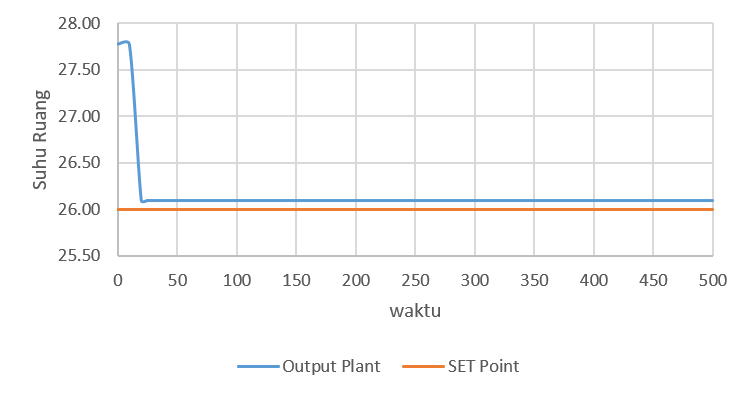
\includegraphics[width=0.75\textwidth]{figures/SimulinkSP1Td}
	\caption{Hasil Simulasi Sistem Kontrol untuk Suhu Ruang SP1}
	\label{fig:5:SimulinkSP1Td}
\end{figure}

\begin{figure}[!h]
	\centering
	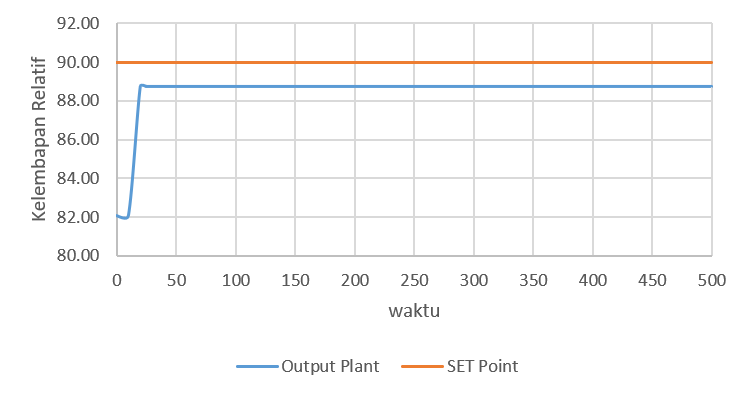
\includegraphics[width=0.75\textwidth]{figures/SimulinkSP1RH}
	\caption{Hasil Simulasi Sistem Kontrol untuk Kelembapan Relatif SP1}
	\label{fig:5:SimulinkSP1RH}
\end{figure}

\begin{figure}[!h]
	\centering
	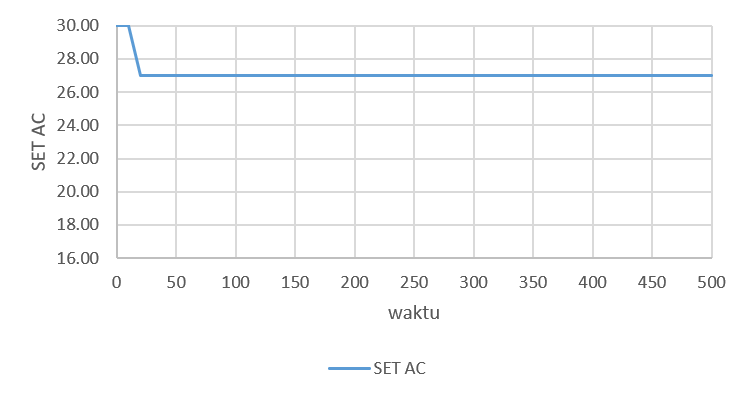
\includegraphics[width=0.75\textwidth]{figures/SimulinkSP1AC}
	\caption{Nilai MV SET AC SP1}
	\label{fig:5:SimulinkSP1AC}
\end{figure}

\begin{figure}[!h]
	\centering
	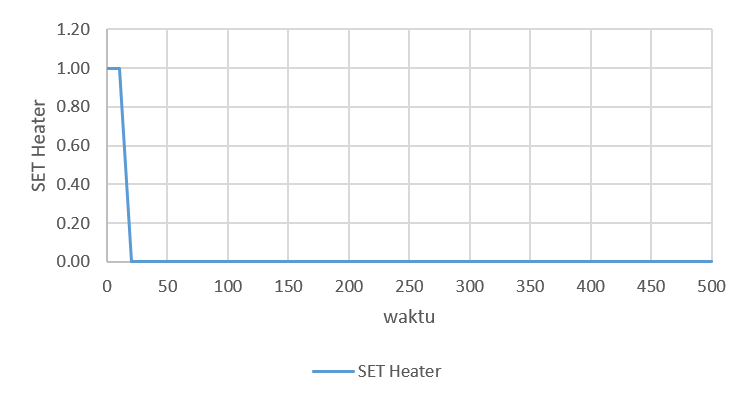
\includegraphics[width=0.75\textwidth]{figures/SimulinkSP1HT}
	\caption{Nilai MV SET Heater SP1}
	\label{fig:5:SimulinkSP1HT}
\end{figure}

\subsubsection{SET POINT Konstan SP2}

Kombinasi SET Point dapat dilihat pada Tabel \ref{tbl:5:SP2Combination}. Hasil dari simulasi simulink dapat dilihat pada Gambar \ref{fig:5:SimulinkSP2Td} dan Gambar \ref{fig:5:SimulinkSP2RH}. Pada Gambar \ref{fig:5:SimulinkSP2Td} dan Gambar \ref{fig:5:SimulinkSP2RH} dapat dilihat bahwa nilai \textit{error steady-state} sistem kontrol cukup kecil. Nilai \textit{Error Steady-State} dari simulasi ini dapat dilihat pada Tabel \ref{tbl:5:SP2Ess}. Grafik dari hasil simulasi dapat dilihat pada Gambar \ref{fig:5:SimulinkSP2Td} untuk Suhu Ruang dan Gambar \ref{fig:5:SimulinkSP2RH} untuk Kelembapan Relatif. Kontroler mengeluarkan nilai \textit{Manipulated Variable} yang ditunjukkan oleh Gambar \ref{fig:5:SimulinkSP2AC} dan Gambar \ref{fig:5:SimulinkSP2HT}.

\vspace{0.5em}
\begin{table}[!h]
	\caption{Nilai Kombinasi SET POINT SP2}
	\label{tbl:5:SP2Combination}
	\centering
	% use packages: array
	\begin{tabular}{|l|c|}
		\hline
		\textbf{Variabel} & \textbf{SET Point} \\ \hline
		Suhu Ruang (Td) & 27$^\circ$C          \\ \hline
		Kelembapan Relatif (RH) & 85\%         \\ \hline
		Suhu Luar (To) & 27$^\circ$C           \\ \hline
		Radiasi Matahari (RD) & 400 W/m$^2$    \\ \hline
	\end{tabular}
\end{table}

\begin{table}[!h]
	\caption{Hasil Simulasi Sistem Kontrol SP2}
	\label{tbl:5:SP2Ess}
	\centering
	% use packages: array
	\begin{tabular}{|l|c|c|c|}
		\hline
		\textbf{Variabel} & \textbf{SET Point} & \textbf{Output Plant} & \textbf{Error Steady-State}\\ \hline
		Suhu Ruang (Td) & 27$^\circ$C & 27,09$^\circ$C & 0,09$^\circ$C \\ \hline
		Kelembapan Relatif (RH) & 85\% & 86,14\% & 1,14\% \\ \hline
	\end{tabular}
\end{table}

\begin{figure}[!h]
	\centering
	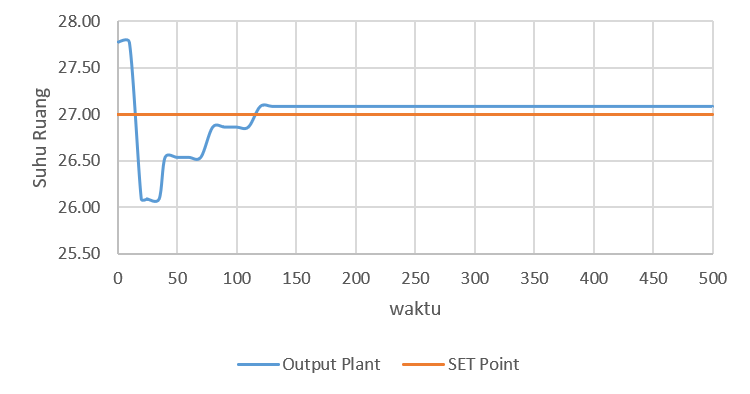
\includegraphics[width=0.75\textwidth]{figures/SimulinkSP2Td}
	\caption{Hasil Simulasi Sistem Kontrol untuk Suhu Ruang SP2}
	\label{fig:5:SimulinkSP2Td}
\end{figure}

\begin{figure}[!h]
	\centering
	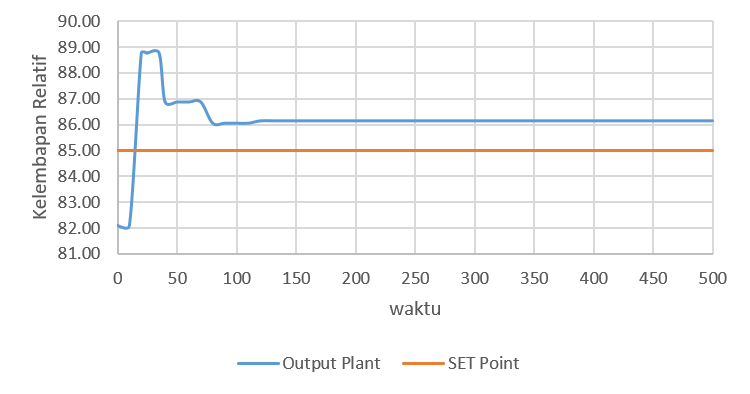
\includegraphics[width=0.75\textwidth]{figures/SimulinkSP2RH}
	\caption{Hasil Simulasi Sistem Kontrol untuk Kelembapan Relatif SP2}
	\label{fig:5:SimulinkSP2RH}
\end{figure}

\begin{figure}[!h]
	\centering
	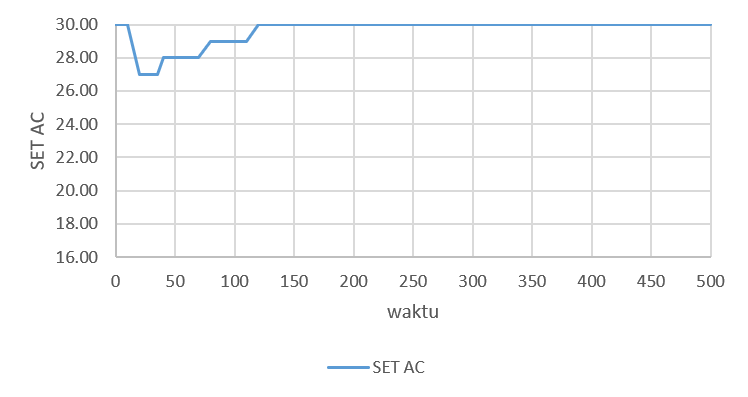
\includegraphics[width=0.75\textwidth]{figures/SimulinkSP2AC}
	\caption{Nilai MV SET AC SP2}
	\label{fig:5:SimulinkSP2AC}
\end{figure}

\begin{figure}[!h]
	\centering
	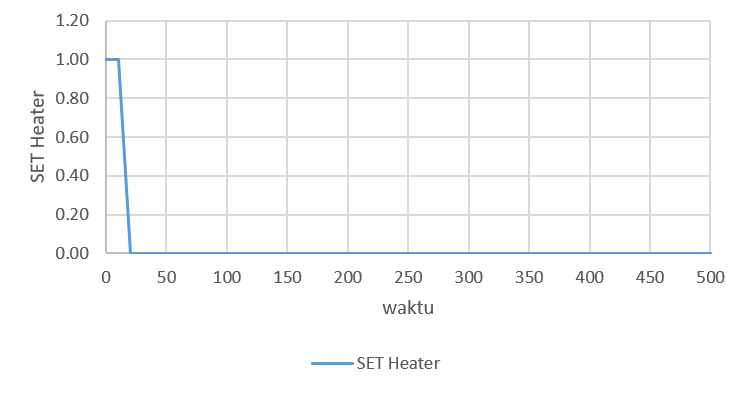
\includegraphics[width=0.75\textwidth]{figures/SimulinkSP2HT}
	\caption{Nilai MV SET Heater SP2}
	\label{fig:5:SimulinkSP2HT}
\end{figure}

\subsubsection{SET POINT Fungsi Step SP3}

Kombinasi SET Point dapat dilihat pada Tabel \ref{tbl:5:SP3Combination}. Hasil dari simulasi simulink dapat dilihat pada Gambar \ref{fig:5:SimulinkSP3Td} dan Gambar \ref{fig:5:SimulinkSP3RH}. Pada Gambar \ref{fig:5:SimulinkSP3Td} dan Gambar \ref{fig:5:SimulinkSP3RH} dapat dilihat bahwa nilai \textit{error steady-state} sistem kontrol cukup kecil. Nilai \textit{Error Steady-State} dari simulasi ini dapat dilihat pada Tabel \ref{tbl:5:SP3Ess}. Grafik dari hasil simulasi dapat dilihat pada Gambar \ref{fig:5:SimulinkSP3Td} untuk Suhu Ruang dan Gambar \ref{fig:5:SimulinkSP3RH} untuk Kelembapan Relatif. Kontroler mengeluarkan nilai \textit{Manipulated Variable} yang ditunjukkan oleh Gambar \ref{fig:5:SimulinkSP3AC} dan Gambar \ref{fig:5:SimulinkSP3HT}.

\begin{table}[!h]
	\caption{Nilai Kombinasi SET POINT SP3}
	\label{tbl:5:SP3Combination}
	\centering
	% use packages: array
	\begin{tabular}{|l|c|}
		\hline
		\textbf{Variabel} & \textbf{SET Point} \\ \hline
		Suhu Ruang (Td) & Step 26$^\circ$C -> 27$^\circ$C \\ \hline
		Kelembapan Relatif (RH) & Step 90\% -> 85\% \\ \hline
		Suhu Luar (To) & 27$^\circ$C           \\ \hline
		Radiasi Matahari (RD) & 400 W/m$^2$    \\ \hline
	\end{tabular}
\end{table}

\begin{figure}[!h]
	\centering
	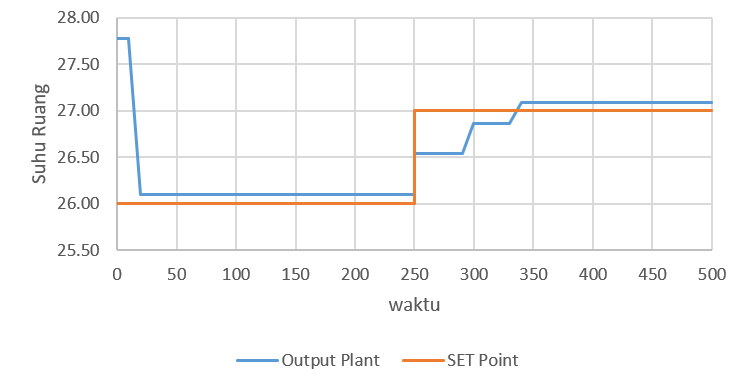
\includegraphics[width=0.75\textwidth]{figures/SimulinkSP3Td}
	\caption{Hasil Simulasi Sistem Kontrol untuk Suhu Ruang SP3}
	\label{fig:5:SimulinkSP3Td}
\end{figure}

\begin{figure}[!h]
	\centering
	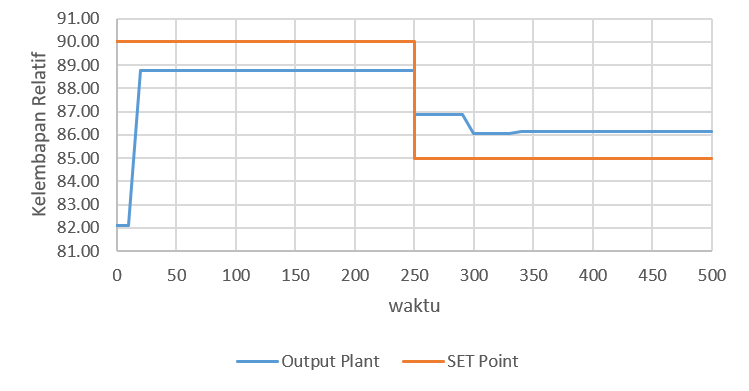
\includegraphics[width=0.75\textwidth]{figures/SimulinkSP3RH}
	\caption{Hasil Simulasi Sistem Kontrol untuk Kelembapan Relatif SP3}
	\label{fig:5:SimulinkSP3RH}
\end{figure}

\begin{figure}[!h]
	\centering
	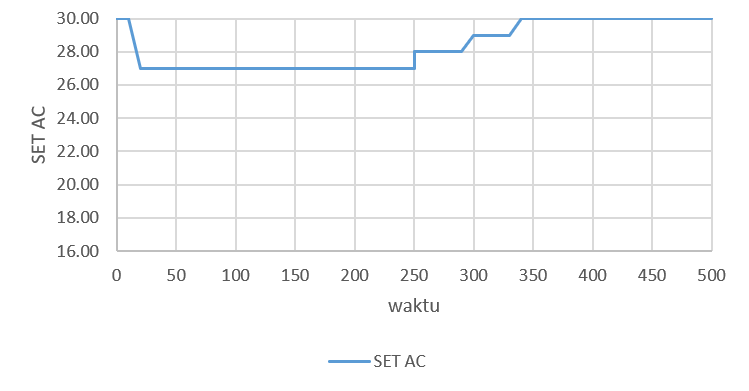
\includegraphics[width=0.75\textwidth]{figures/SimulinkSP3AC}
	\caption{Nilai MV SET AC SP3}
	\label{fig:5:SimulinkSP3AC}
\end{figure}

\begin{figure}[!h]
	\centering
	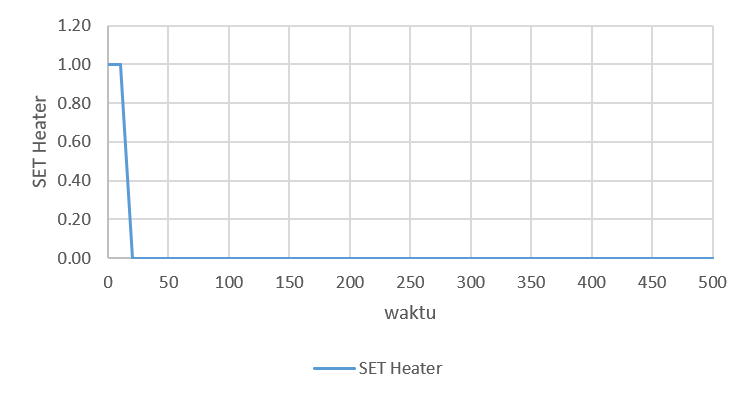
\includegraphics[width=0.75\textwidth]{figures/SimulinkSP3HT}
	\caption{Nilai MV SET Heater SP3}
	\label{fig:5:SimulinkSP3HT}
\end{figure}